\section{Experiments on a laboratory shaker - Test 1}
\label{sec:shaker_test01}

After the \gls{pc} implementation of the framework has been tested widely on the \gls{ims} dataset, the \gls{glo:edge} implementation had to be validated experimentally. The first test was done with a laboratory shaker, which is basically a powerful active speaker with a really wide band that can be attached with a bolt to a structure, to vibrate it.

In this case, an accelerometer, whose key specifications are shown in \autoref{tab:adxl335_specifications}, was used to capture the vibration signal. The accelerometer was attached to the shaker, with a custom 3D-printed fixture. This first test has the scope of checking the capability of the \gls{glo:edge} implementation to detect a new low amplitude harmonic in the signal. The signal is generated as a \texttt{.wav} file and fed to the shaker by a player. Both the input of the shaker and the output of the accelerometer were monitored with a digital oscilloscope. The setup is shown in \autoref{fig:shaker_setup}.



\begin{table}[h]
    \centering
    \caption{Specifications of the ADXL335 Accelerometer}
    \label{tab:adxl335_specifications}
    \begin{tabular}{ll} 
    \toprule
    \textbf{Parameter} & \textbf{Value} \\ 
    \hline
    Supply Voltage & 1.8V to 3.6V \\
    Sensing Range & ±3g \\
    Sensitivity & 300 mV/g \\
    Bandwidth & 0.5 Hz to 1600 Hz \\
    Output Type & Analog \\
    Output Voltage Range & 0V to V$_{CC}$ \\
    Operating Temperature & -40°C to +85°C \\
    Package & $3\si{mm} \times 5 \si{mm} \times 1 \si{mm}$ \\
    \bottomrule
    \end{tabular}
\end{table}

\begin{figure}
    \centering
    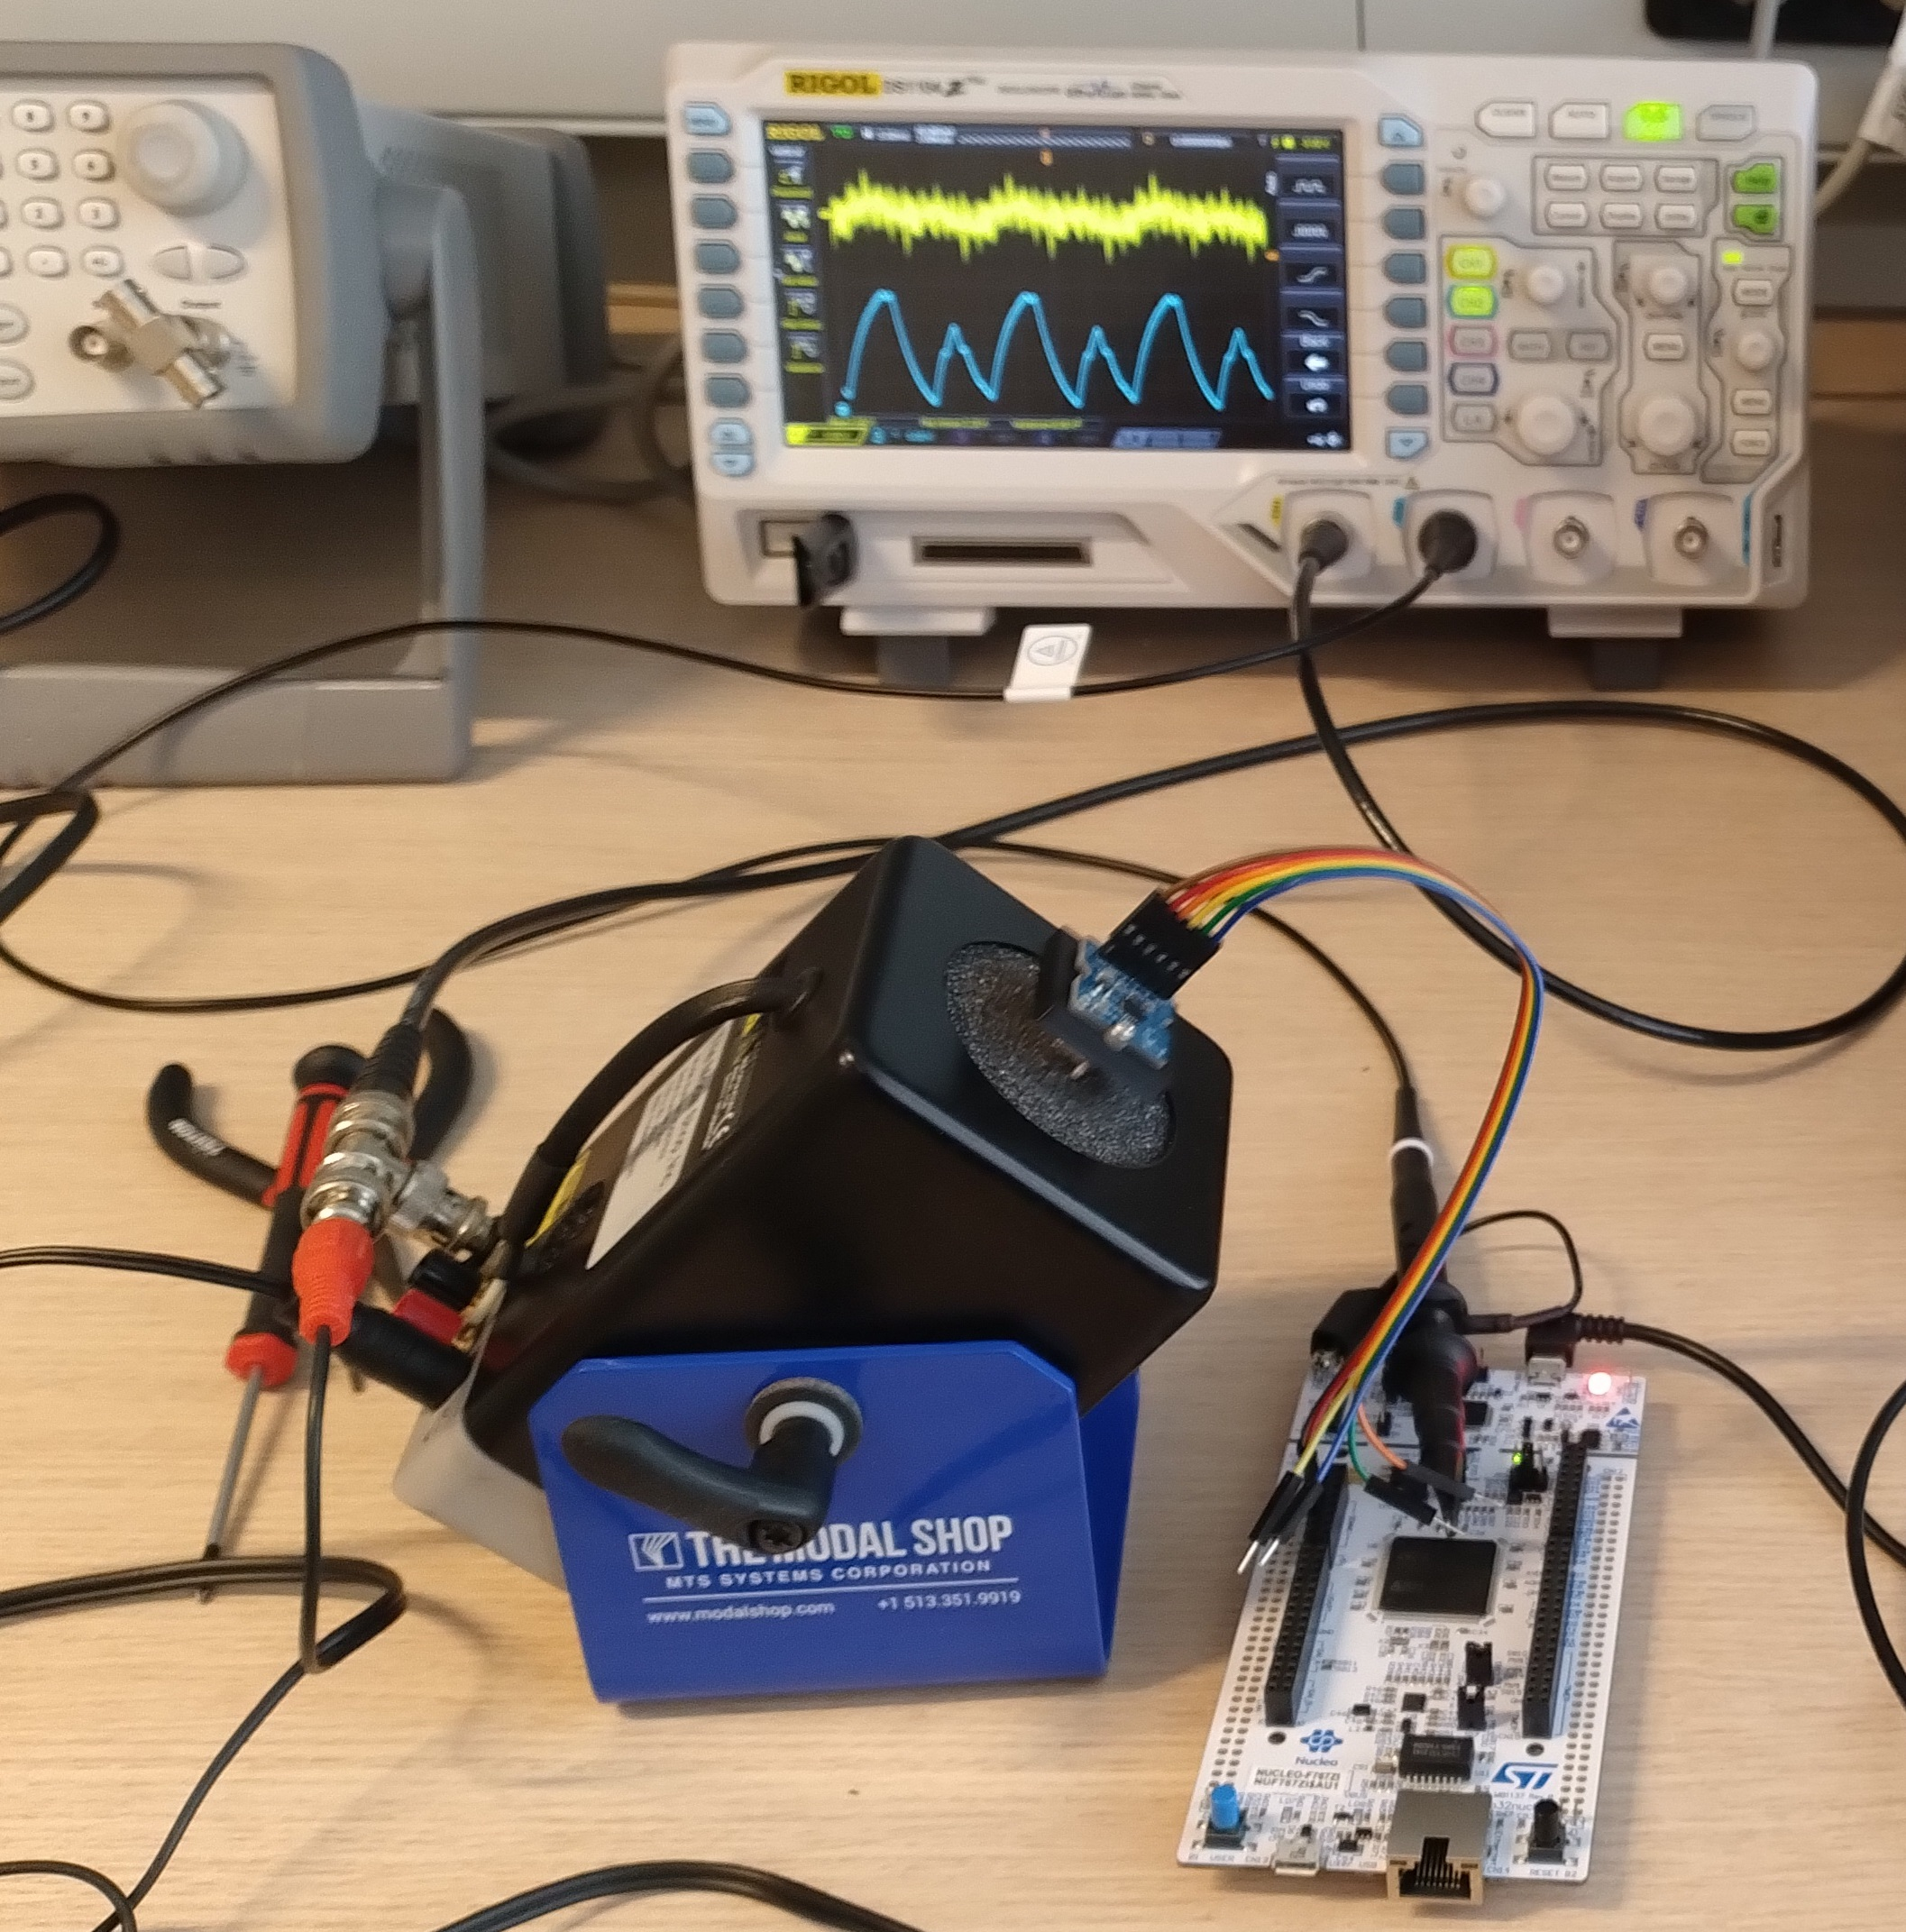
\includegraphics[width=.4\textwidth]{Images/shaker/IMG_20231207_103126143.jpg}
    \caption{Setup of the shaker tests.}
    \label{fig:shaker_setup}
\end{figure}
\begin{table}
    \centering
    \caption{Harmonic coefficients for the shaker test. Wave 1 and Wave 2 are training signals, and Harmonic Injection is the signal to be detected.}
    \label{tab:shaker_param_01}
    \begin{tabular}{lccccccc} 
    \toprule
    \multirow{2}{*}{\textbf{Signal Name }} & \multicolumn{6}{c}{\textbf{Harmonic frequency} [Hz]} & \multirow{2}{*}{\textbf{Amplitude} [mV]$_{pp}$} \\
     & 30 & 70 & 100 & 300 & 800 & 1400 &  \\ 
    \hline
    Wave 1 & 0.1 & 1.0 & 1.0 & \multicolumn{1}{c}{-} & 1.0 & 1.0 & 1000 \\
    Wave 2 & 0.1 & 0.8 & 1.0 & \multicolumn{1}{c}{-} & 3.0 & 0.6 & 1000 \\
    Harmonic Injection & 0.1 & 1.0 & 1.0 & 0.1 & 1.0 & 1.0 & 1000 \\
    \bottomrule
    \end{tabular}
    \end{table}

\subsection{Training and evaluating}
The framework was firstly set to gather the data, extract the features according to the configuration, and send the data to the \gls{pc} for training. The training signals are two waves with different harmonic content and the test signal is very similar to one used for training, except for the presence of an additional harmonic with a small amplitude. The train and test signals harmonic content is reported in \autoref{tab:shaker_param_01}. The amplitude of the vibration has been tuned at each test to ensure that the microcontroller was reading a signal of 1V$_{pp}$. The amplitude of the signals has been kept constant to test the capability of the framework to detect the frequency content of the signal in the feature extraction phase. The waveform of the test signals is shown with the one of one training signal in \autoref{fig:shaker}, to show the similarity of the two signals. 

The setting of the framework can be resumed as follows:
\begin{itemize}
    \item 67 features extracted from the signal ($2^6=64$ features from the wavelet decomposition, mean, P2P, and \gls{rms});
    \item 110 samples for training for each signal.
    \item sampling frequency of 5kHz, for 1s of acquisition.
\end{itemize}

After the data gathering was completed, the training was done on the \gls{pc}, as usual. The silhouette score correctly suggested 2 as the best number of \gls{glo:clust}s to be used. The \gls{pc} part of the framework outputs the \texttt{model.h} file directly in the embedded project folder, so just a new upload of the firmware was needed to test the detection. The microcontroller was then set in \emph{evaluation} mode and both the two training signals and the test signal were fed to the shaker. 

\subsection{Results}
The result of the novelty detection is shown in \autoref{fig:shaker_results}. The result is consistent with the expected outcome, as the training signals produced a negative novelty metric, while the test signal produced a positive (and quite high) novelty metric. The spectrum of the signals used is shown graphically in \autoref{fig:shaker_spectrum}.

\begin{figure}
    \centering
    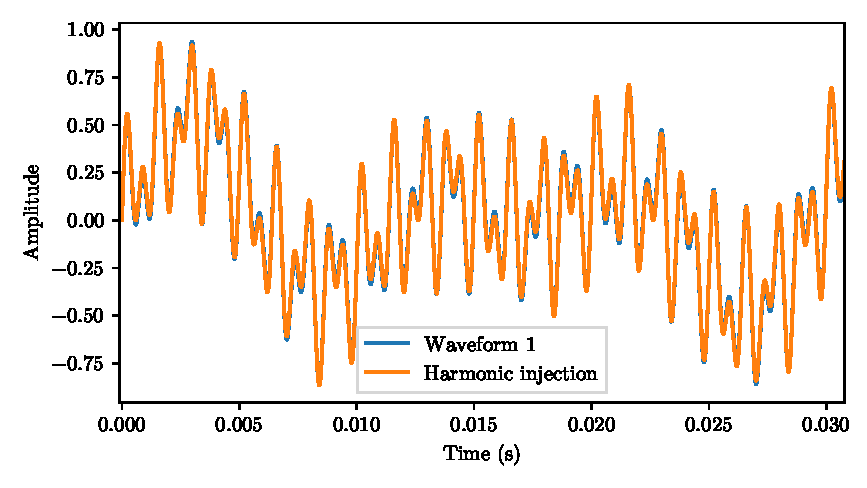
\includegraphics{Images/shaker/Figure_1.pdf}
    \caption{Waveform comparison of the shaker test.}
    \label{fig:shaker}
\end{figure}

\begin{figure}
    \centering
    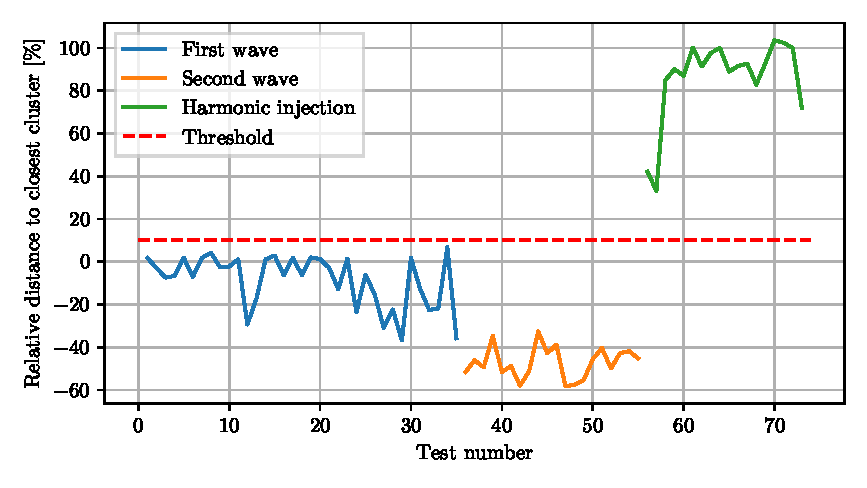
\includegraphics{Images/shaker/Results.pdf}
    \caption{Novelty detection result}
    \label{fig:shaker_results}
\end{figure}

\begin{figure}
    \centering
    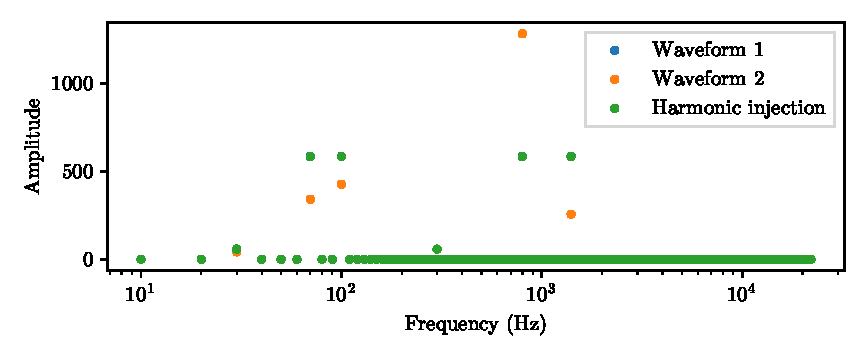
\includegraphics{Images/shaker/spectrum.pdf}
    \caption{Spectrum of the waveforms.}
    \label{fig:shaker_spectrum}
\end{figure}


